% Options for packages loaded elsewhere
\PassOptionsToPackage{unicode}{hyperref}
\PassOptionsToPackage{hyphens}{url}
%
\documentclass[
]{book}
\title{PreCalculus 12 Minibook}
\author{Joshua Zhang}
\date{}

\usepackage{amsmath,amssymb}
\usepackage{lmodern}
\usepackage{iftex}
\ifPDFTeX
  \usepackage[T1]{fontenc}
  \usepackage[utf8]{inputenc}
  \usepackage{textcomp} % provide euro and other symbols
\else % if luatex or xetex
  \usepackage{unicode-math}
  \defaultfontfeatures{Scale=MatchLowercase}
  \defaultfontfeatures[\rmfamily]{Ligatures=TeX,Scale=1}
\fi
% Use upquote if available, for straight quotes in verbatim environments
\IfFileExists{upquote.sty}{\usepackage{upquote}}{}
\IfFileExists{microtype.sty}{% use microtype if available
  \usepackage[]{microtype}
  \UseMicrotypeSet[protrusion]{basicmath} % disable protrusion for tt fonts
}{}
\makeatletter
\@ifundefined{KOMAClassName}{% if non-KOMA class
  \IfFileExists{parskip.sty}{%
    \usepackage{parskip}
  }{% else
    \setlength{\parindent}{0pt}
    \setlength{\parskip}{6pt plus 2pt minus 1pt}}
}{% if KOMA class
  \KOMAoptions{parskip=half}}
\makeatother
\usepackage{xcolor}
\IfFileExists{xurl.sty}{\usepackage{xurl}}{} % add URL line breaks if available
\IfFileExists{bookmark.sty}{\usepackage{bookmark}}{\usepackage{hyperref}}
\hypersetup{
  pdftitle={PreCalculus 12 Minibook},
  pdfauthor={Joshua Zhang},
  hidelinks,
  pdfcreator={LaTeX via pandoc}}
\urlstyle{same} % disable monospaced font for URLs
\usepackage{longtable,booktabs,array}
\usepackage{calc} % for calculating minipage widths
% Correct order of tables after \paragraph or \subparagraph
\usepackage{etoolbox}
\makeatletter
\patchcmd\longtable{\par}{\if@noskipsec\mbox{}\fi\par}{}{}
\makeatother
% Allow footnotes in longtable head/foot
\IfFileExists{footnotehyper.sty}{\usepackage{footnotehyper}}{\usepackage{footnote}}
\makesavenoteenv{longtable}
\usepackage{graphicx}
\makeatletter
\def\maxwidth{\ifdim\Gin@nat@width>\linewidth\linewidth\else\Gin@nat@width\fi}
\def\maxheight{\ifdim\Gin@nat@height>\textheight\textheight\else\Gin@nat@height\fi}
\makeatother
% Scale images if necessary, so that they will not overflow the page
% margins by default, and it is still possible to overwrite the defaults
% using explicit options in \includegraphics[width, height, ...]{}
\setkeys{Gin}{width=\maxwidth,height=\maxheight,keepaspectratio}
% Set default figure placement to htbp
\makeatletter
\def\fps@figure{htbp}
\makeatother
\setlength{\emergencystretch}{3em} % prevent overfull lines
\providecommand{\tightlist}{%
  \setlength{\itemsep}{0pt}\setlength{\parskip}{0pt}}
\setcounter{secnumdepth}{5}
\usepackage{booktabs}

\newenvironment{cols}[1][]{}{}

\newenvironment{col}[1]{\begin{minipage}{#1}\ignorespaces}{%
\end{minipage}
\ifhmode\unskip\fi
\aftergroup\useignorespacesandallpars}

\def\useignorespacesandallpars#1\ignorespaces\fi{%
#1\fi\ignorespacesandallpars}

\makeatletter
\def\ignorespacesandallpars{%
  \@ifnextchar\par
    {\expandafter\ignorespacesandallpars\@gobble}%
    {}%
}
\makeatother
\ifLuaTeX
  \usepackage{selnolig}  % disable illegal ligatures
\fi

\usepackage{amsthm}
\newtheorem{theorem}{Theorem}[chapter]
\newtheorem{lemma}{Lemma}[chapter]
\newtheorem{corollary}{Corollary}[chapter]
\newtheorem{proposition}{Proposition}[chapter]
\newtheorem{conjecture}{Conjecture}[chapter]
\theoremstyle{definition}
\newtheorem{definition}{Definition}[chapter]
\theoremstyle{definition}
\newtheorem{example}{Example}[chapter]
\theoremstyle{definition}
\newtheorem{exercise}{Exercise}[chapter]
\theoremstyle{definition}
\newtheorem{hypothesis}{Hypothesis}[chapter]
\theoremstyle{remark}
\newtheorem*{remark}{Remark}
\newtheorem*{solution}{Solution}
\begin{document}
\maketitle

{
\setcounter{tocdepth}{1}
\tableofcontents
}
\hypertarget{preface}{%
\chapter*{Preface}\label{preface}}
\addcontentsline{toc}{chapter}{Preface}

This minibook (unfinished) summarizes the key concepts and common examples in Pre-Calculus 12 to aid students in learning and reviewing. The content follows the curriculum in BC, Canada.

\hypertarget{motivation}{%
\section*{Motivation}\label{motivation}}
\addcontentsline{toc}{section}{Motivation}

In the multimedia dominated world today, there are plenty of tutorial videos that you can just watch and learn math.

Why do you need to read a book?

As a college and high school educator, I have noticed an unfavorable learning habit among students: purpose-driven. This leads to impatience and ``learning without thinking.'' Students often fail to see how the topics covered in a given course are interconnected and may not understand the reasoning behind the specific order in which the topics are presented. Believe it or not, the learning outcome (and the final grade, of course) is highly correlated to how the student understands the ``big image'' of a course. In other words, the interconnections between topics are very important, especially for subjects like mathematics, which usually has topics built upon the previous ones.

In my opinion, reading a textbook could greatly help a student to get the ``big image,'' because when you turn the pages (physical book) or scroll down the document or table of content (e-book) to the topic your are currently learning, you enhance your sense of the order of the topics, in particular the previous chapter or section. For example, if you are learning ``subtracting numbers'' in elementary school, you may keep seeing ``adding numbers'' right before it, so that you know that ``subtraction'' is build upon ``addition'' as you have to kind of understand ``subtraction'' as something like ``reverting the addition.''

However, a full textbook could be a little too long and redundant for students to read (although this should still be the goal). We can go half a step backward and start with this \emph{minibook}. While the overall sense of the topics and their interconnections are preserved, the contents are not too redundant to overload your mind. Only key concepts and very common examples are included in this minibook; the conclusions come first, so you can skip the explanations if you don't want understand them (although this is highly discouraged). Furthermore, this minibook could also serve as a perfect review material given its compactness.

\hypertarget{how-to-read-this-minibook}{%
\section*{How to Read This Minibook}\label{how-to-read-this-minibook}}
\addcontentsline{toc}{section}{How to Read This Minibook}

This \emph{minibook} is different from a common textbook in several ways. As a result, you can take advantage of them by reading \emph{wisely}.

\begin{itemize}
\tightlist
\item
  Free of redundant long paragraphs, instead, point forms and list are frequently used to organize the key points.

  \begin{itemize}
  \tightlist
  \item
    This means the contents are already abridged so that only those important remains.
  \item
    As a student, you should not skip any sections/paragraphs.
  \end{itemize}
\item
  Collapsible sections including examples, proofs of theorems, etc. allows readers to read selectively.

  \begin{itemize}
  \tightlist
  \item
    Make good use of this feature by not expand a collapsed section until you really need to.
  \item
    For example, if the answer is in a collapsed section (hidden), you should try to work on solving the problem yourself before expanding the section to see the answer.
  \end{itemize}
\item
  Interactive table of contents for fast navigation and clear connections through topics.

  \begin{itemize}
  \tightlist
  \item
    You can easily find a topic in the table of contents on the left side.
  \item
    When you are reading through a chapter, the focus on the table of contents automatically changes as you scrolls down. This allows you to keep track on your progress.
  \end{itemize}
\end{itemize}

\hypertarget{how-to-learn-math}{%
\section*{How to Learn Math}\label{how-to-learn-math}}
\addcontentsline{toc}{section}{How to Learn Math}

Personally, I would divide the learning process of a mathematical concept (and perhaps many other concepts) into the following stages:

\begin{enumerate}
\def\labelenumi{\arabic{enumi}.}
\tightlist
\item
  Getting to know the concept. In this beginning stage, we have just heard about or read about the new concept.
\item
  Accepting the concept. This is the stage where we find the concept ``making sense.''
\item
  Applying the concept to a common scenario. We can solve a common problem using the concept, despite that we may not know why it is so. When the problem is tricky or involves special case, we may still get confused. \emph{This is the stage where most students stop going further}.
\item
  Deriving the concept. In this stage, we start to think how this concept was originally discovered/emerged/derived.
\item
  Understanding and/or proving the concept. As we are able to derive the concept and understand why it is necessary in math (such as how it might serve the development of mathematics by supporting/preparing for other concepts).
\item
  Exploring the concept. This is the stage where we seriously learn math. Although mathematics has already been well developed, which means that the chance of discovering a new concept is low, it is still a great practice to try to use the concepts that we understand to explore new concepts. If you find the a new concept through exploration, most likely you will find it in a future math course, but this means that you could be a mathematician if you were born hundreds of years ago!
\end{enumerate}

I will use an example to further explain these stages. Let's say I am learning about \emph{system of two equations}.

\begin{enumerate}
\def\labelenumi{\arabic{enumi}.}
\tightlist
\item
  I know how to solve for \(x\) in one equation. Now there are two equations, and there are both \(x\) and \(y\) to solve for.
\item
  When I look at the teacher solving a system of equations, I see how it works. I think I know how to use the elimination method and the substitution method. I also remember that the solution is the intersection of the two lines, although I don't know what this means.
\item
  After getting stuck a few times and resolving my confusion through reading notes/asking for help, I can solve for a system of two equations by myself now. I simply remember and follow the steps that the teacher/textbook tells me.
\item
  I wonder how the elimination method works, in particular why can I subtract/add two equations altogether? Also, how is the system related to the two lines in a coordinate plane?
\item
  I reviewed the properties of equations, and realized that an equation has its left side and right side being equal in values. So, if we add two equations together, the sum of each side of them would also be equal, which makes the sum also an equation. Regarding to the graph, I understand that all points on a curve satisfy the corresponding equation, so if a point is on both the two lines, it satisfies both equations, thus it is the solution to the system. Furthermore, a system of equations with no solution involves two parallel lines that no point is on both of them; a system of equations with infinitely many solution includes two equations that represent the same line. I might be able to write a more formal proof to show this.
\item
  What happens if we have three equations from which we solve for \(x\), \(y\), and \(z\)? How would it relate to lines in the three dimensional space? How about 4 equations? Is there a four dimensional space in the real world or in mathematics? How about \(n\) equations? How does the number of equations and the number of unknowns affect the result? We are going towards the college level \emph{Linear Algebra} from there on.
\end{enumerate}

Stopping at stage 3 is fine if your purpose is just getting a good grade in this course. In this case, you may skip the optional proofs in this minibook. However, if you intend to learn mathematics or related subjects (physics, computer science, economics, statistics, etc.) in university, or if you want to , I would highly recommend that you to go further to stage 5.

Learning requires patience and time. There is nothing in the world that you can learn in no time. Keep in mind that you have to go through the stages in order, which means you never start from understanding anything, but start from applying it. This might sound counter-intuitive, but consider the process of learning to bike for example. Do you understand why a bike does not fall before you can ride it? Put another way, being able to ride a bike would greatly help you in understanding why it does not fall. This is why some people say ``\emph{you don't understand math, you get used to it}.'' Summarizing all the above, the most important thing in learning math is \emph{practicing}.

\hypertarget{about-the-author}{%
\section*{About the Author}\label{about-the-author}}
\addcontentsline{toc}{section}{About the Author}

I have been helping students learning mathematics and many other science subjects for more than ten years. I went to school in China before university. Then, I got my bachelors degree in Mathematics and in Physics from University of Colorado at Boulder, and I got my master degree in Material Science and Engineering from the same school. After graduation, I started to work as a math and science tutor in Vancouver, Canada.

Unlike teaching in a classroom, private tutoring allowed me to know how students learn in much more details, especially for the students who are struggling with math. Besides the learning habits of the students, I also had the chance to know about the teaching style of the teachers in schools from the perspective of the students. I realized that most students never read the textbooks for their math classes; in fact, neither do many math teachers use textbooks now. Personally, I highly value the importance of a textbook as it not only provides students with the necessary knowledge, but also outlines the topics in the order that shows how they connect and relate. However, when I was trying to recommend a textbook to students learning pre-calculus/high school math in BC, I could not find one that is good and compact -- students do not wish to ``waste'' too much time on reading. These summarize the reasons that led me to writing this minibook.

When reading this minibook, if you have any suggestions, concerns, questions, or if you find any mistakes, please do not hesitate to \href{https://www.miracleeducation.ca/contact/}{contact me}.

\hypertarget{reviewprerequisite}{%
\chapter*{Review/Prerequisite}\label{reviewprerequisite}}
\addcontentsline{toc}{chapter}{Review/Prerequisite}

This chapter summarizes what you are expected to know before reading this minibook, or take pre-calculus 12.

\hypertarget{sets}{%
\section{Sets}\label{sets}}

\hypertarget{introduction-and-definition}{%
\subsection{Introduction and Definition}\label{introduction-and-definition}}

\begin{definition}
\protect\hypertarget{def:set}{}\label{def:set}A \textbf{set} is a collection of \emph{different} objects, called \textbf{elements} of the set. Usually, sets are denoted by capital letters such as \(A\), \(B\), etc. The elements of a set can be numbers or other objects such as vectors, functions, other sets, etc. We write \(a \in A\) if the set \(A\) contains the element \(a\), and we read ``\(a \in A\)'' as ``\(\boldsymbol{a}\) \textbf{is an element of} \(\boldsymbol{A}\).''
\end{definition}

The \textbf{empty set} is the set with no element, denoted as \(\varnothing\).

A set can have finitely many elements, called a \textbf{finite set}, or infinitely many elements, called an \textbf{infinite set}.

\begin{example}
\protect\hypertarget{exm:roster}{}\label{exm:roster}\(A = \{\text{red},\, \text{green},\, \text{blue}\}\), \(B = \{1,\,2,\,3,\,4,\,5\}\), and \(C = \{1,\,2,\,3,\,\dots\}\) are all examples of sets. Here, \(A\) and \(B\) are finite sets, and \(C\) is an infinite set.\\
The set \(A\) has 3 elements, red, green, and blue. So, \(\text{red} \in A\), \(\text{green} \in A\), and \(\text{blue} \in A\). Similarly, \(1 \in B\), \(2 \in B\), etc.
\end{example}

In this minibook, we will only see sets with numerical elements.

\hypertarget{notations}{%
\subsection{Notations}\label{notations}}

To define a set, we can list the elements one by one or describe the elements in words and/or math. The methods of defining a set are summarized as follows:

\begin{itemize}
\item
  \textbf{Roster Notation}/\textbf{Enumeration Notation} (Listing the elements)\\
  All the three sets in Example \ref{exm:roster} are defined under the roster notation.
\item
  \textbf{Semantic Notation}/\textbf{Statement Notation} (Describing the properties of the elements in words)

  \begin{example}
  \protect\hypertarget{exm:semantic}{}\label{exm:semantic}\(D\) is the set of all positive integers less than 100; \(E\) is the set of all students in my pre-calculus 12 class.
  \end{example}
\item
  \textbf{Set Builder Notation} (Describing the properties of the elements in math and/or words)\\
  State the symbol to be described on the left side of ``\(\,\mid\,\)'' or ``\(\,:\,\)'' then describe the symbol on the right side.

  \begin{example}
  \protect\hypertarget{exm:set-builder}{}\label{exm:set-builder}

  The following sets are defined using the set builder notation:
  \begin{align*}
  F &= \{x \mid x \in D \text{ and $x$ is a multiple of } 2\} = \{x \in D \mid x \text{ is a multiple of } 10\}\\
  G &= \{n \mid n^2 \in D\}\\
  H &= \{x^2 \mid x \in B\} = \{x \mid x = b^2 \text{ for some } b \in B\}
  \end{align*}

  See the roster notation of the sets \(F,\,G,\,H\) to check your understanding

  \begin{align*}
  F &= \{10,\, 20,\, \dots,\, 90\}\\
  G &= \{1,\, 2,\, 3,\, \dots,\, 9\}\\
  H &= \{1,\, 4,\, 9,\, 16,\, 25\}
  \end{align*}

  \end{example}
\item
  \textbf{Interval Notation} (only for sets of connected real numbers)\\
  An interval is written as two numbers separated by a comma, surrounded by round or square bracket The smaller of the two numbers is always on the left. The interval is the set of all real numbers between these two numbers, with each of the two numbers themselves \emph{included} if a \emph{square bracket} is used, or \emph{excluded} if a \emph{round bracket} (parenthesis) is used. The two numbers are called the \textbf{endpoints} of the interval.

  \begin{example}
  \protect\hypertarget{exm:interval}{}\label{exm:interval}The following intervals are described in set builder notation.
  \begin{align*}
  I_1 &= (1,\, 3) = \{x \in \mathbb{R} \mid 1 < x < 3\}\\
  I_2 &= [-2,\, 2] = \{x \in \mathbb{R} \mid -2 \le x \le 2\}\\
  I_3 &= [0,\, 5) = \{x \in \mathbb{R} \mid 0 \le x < 5\}\\
  I_4 &= (0,\, 5] = \{x \in \mathbb{R} \mid 0 < x \le 5\} .
  \end{align*}
  \end{example}

  An interval is \textbf{open} if both the two endpoints are excluded in the interval, such as \(I_1\); an interval is \textbf{closed} if both the two endpoints are included, such as \(I_2\); an interval is \textbf{half-open} if exactly one endpoint is included, such as \(I_3\) (right-opened) and \(I_4\) (left-open).

  \begin{example}
  \protect\hypertarget{exm:inf-interval}{}\label{exm:inf-interval}An interval can be bounded on only one side:
  \begin{align*}
  I_5 &= (-1,\, \infty) = \{x \in \mathbb{R} \mid x > -1\}\\
  I_6 &= (-\infty,\, 3] = \{x \in \mathbb{R} \mid x \le 3\} .
  \end{align*}
  \end{example}

  Note that the symbol \(\infty\), which means \emph{infinity}, is \emph{not} a number and thus can \emph{never} be included in an interval.
\end{itemize}

\hypertarget{subset}{%
\subsection{Subset}\label{subset}}

\begin{definition}
\protect\hypertarget{def:subset}{}\label{def:subset}We say the set \(P\) is a \emph{subset} of the set \(Q\) (written as \(P \subseteq Q\)) if all elements in \(P\) are also in \(Q\).
\end{definition}

\begin{example}
\protect\hypertarget{exm:subset1}{}\label{exm:subset1}Recall from Example \ref{exm:roster}, \(B = \{1,\, 2,\, 3,\, 4,\, 5\}\) and \(C = \{1,\, 2,\, 3,\, \dots\}\). All elements in \(B\) are in \(C\), so \(B \subseteq C\).
\end{example}

\begin{example}
\protect\hypertarget{exm:subset2}{}\label{exm:subset2}Recall from Example \ref{exm:semantic}, \(D = \{1,\, 2,\, \dots,\, 99\}\), and from Example \ref{exm:set-builder}, \(F = \{10,\, 20,\, \dots,\, 90\}\) and \(G = \{1,\, 2,\, \dots,\, 9\}\). Both \(F\) and \(G\) are subsets of \(D\).
\end{example}

\begin{example}
\protect\hypertarget{exm:subset3}{}\label{exm:subset3}By definition, every set is a subset of itself. Also, the empty set \(\varnothing\) is a subset of every set.
\end{example}

\hypertarget{basic-set-operations}{%
\subsection{Basic Set Operations}\label{basic-set-operations}}

\hypertarget{union-of-two-sets}{%
\subsubsection{Union of two sets}\label{union-of-two-sets}}

\begin{definition}
\protect\hypertarget{def:union}{}\label{def:union}The \emph{union} of the sets \(P\) and \(Q\) (denoted as \(P \cup Q\)) is the set containing all the elements in either or both \(P\) and \(Q\).
\end{definition}

\begin{example}
\protect\hypertarget{exm:union}{}\label{exm:union}Let's start from the union of some simple sets:
\begin{align*}
& \{1,\, 2,\, 3\} \cup \{1,\, 3,\, 5,\, 7\} = \{1,\, 2,\, 3,\, 5,\, 7\} \\
& \{2,\, 4\} \cup \{10\} = \{2,\, 4,\, 10\} \\
& \{3,\, 6,\, 9\} \cup \{3,\, 6,\, 9\} = \{3,\, 6,\, 9\} .
\end{align*}
\end{example}

\begin{example}
\protect\hypertarget{exm:union-interval}{}\label{exm:union-interval}The union of intervals will appear frequently in this minibook, such as
\begin{align*}
& (-\infty,\, 0] \cup [2,\, 5] = \{x \in \mathbb{R} \mid x \le 0 \text{ or } 2 \le x \le 5\} \\
& (-\infty,\, 3) \cup (3,\, \infty)  = \{x \in \mathbb{R} \mid x \ne 3\} .
\end{align*}
\end{example}

\hypertarget{intersection-of-two-sets}{%
\subsubsection{Intersection of two sets}\label{intersection-of-two-sets}}

\begin{definition}
\protect\hypertarget{def:intersection}{}\label{def:intersection}The \emph{intersection} of the sets \(P\) and \(Q\) (denoted as \(P \cap Q\)) is the set containing only the elements in both \(P\) and \(Q\).
\end{definition}

\begin{example}
\protect\hypertarget{exm:intersection}{}\label{exm:intersection}Let's work with the same simple sets as above:
\begin{align*}
& \{1,\, 2,\, 3\} \cap \{1,\, 3,\, 5,\, 7\} = \{1,\, 3\} \\
& \{2,\, 4\} \cap \{10\} = \varnothing \\
& \{3,\, 6,\, 9\} \cap \{3,\, 6,\, 9\} = \{3,\, 6,\, 9\} .
\end{align*}
\end{example}

\hypertarget{difference-of-two-sets}{%
\subsubsection{Difference of two sets}\label{difference-of-two-sets}}

\begin{definition}
\protect\hypertarget{def:set-diff}{}\label{def:set-diff}The \emph{difference} of the sets \(P\) and \(Q\) (denoted as \(P \setminus Q\) or \(P - Q\)) is the set containing the elements in \(P\) that are not in \(Q\).
\end{definition}

\begin{example}
\protect\hypertarget{exm:set-diff}{}\label{exm:set-diff}Let's work with the same simple sets again:
\begin{align*}
& \{1,\, 2,\, 3\} \setminus \{1,\, 3,\, 5,\, 7\} = \{2\} \\
& \{2,\, 4\} \setminus \{10\} = \{2,\, 4\} \\
& \{3,\, 6,\, 9\} \setminus \{3,\, 6,\, 9\} = \varnothing .
\end{align*}
\end{example}

\hypertarget{common-number-sets}{%
\subsection{Common Number Sets}\label{common-number-sets}}

We will be frequently using these sets in this minibook:

\begin{itemize}
\tightlist
\item
  The set of natural numbers \(\mathbb{N} = \{1,\, 2,\, 3,\, \dots\}\) includes all positive integers (some texts include \(0\) in \(\mathbb{N}\)).
\item
  The set of integers \(\mathbb{Z} = \{\dots,\, -2,\, -1,\, 0,\, 1,\, 2,\, \dots\}\).
\item
  The set of rational numbers \(\displaystyle\mathbb{Q} = \left\{\left.\frac{a}{b}\,\right\vert\, a,b \in \mathbb{Z} \text{ and } b \ne 0 \right\}\) includes all integers and fractions of integers.
\item
  The set of real numbers \(\mathbb{R}\) includes all the numbers on a continuous number line. This includes rational and irrational numbers (all numbers that we have learned until know are real numbers).
\end{itemize}

It might be worth nothing that \(\mathbb{N} \subseteq \mathbb{Z} \subseteq \mathbb{Q} \subseteq \mathbb{R}\).

\hypertarget{operations}{%
\section{Operations}\label{operations}}

\hypertarget{types-of-operations}{%
\subsection{Types of operations}\label{types-of-operations}}

\begin{itemize}
\item
  \textbf{\href{https://en.wikipedia.org/wiki/Addition}{Addition}}, \textbf{\href{https://en.wikipedia.org/wiki/Subtraction}{subtraction}}, \textbf{\href{https://en.wikipedia.org/wiki/Multiplication}{multiplication}}, and \textbf{\href{https://en.wikipedia.org/wiki/Division_(mathematics)}{division}}.
\item
  \textbf{\href{https://en.wikipedia.org/wiki/Exponentiation}{Exponentiation}}, including with negative and fractional exponents

  \begin{itemize}
  \item
    Identities/laws of exponents:

    \begin{itemize}
    \tightlist
    \item
      \(a^{m+n} = a^m \cdot a^n\);
    \item
      \(a^{m-n} = \displaystyle\frac{a^m}{a^n}\), where \(a \ne 0\);
    \item
      \(\left(a^m\right)^n = a^{mn} = \left(a^n\right)^m\);
    \item
      \((ab)^m = a^mb^m\), and \(\displaystyle\left(\frac{a}{b}\right)^m = \frac{a^m}{b^m}\), where \(b \ne 0\);
    \item
      \(a^0 = 1\) whenever \(a \ne 0\) (what is \(0^0\)?).
    \end{itemize}
  \item
    Converting a negative exponent:
    \[a^{-m} = \frac{1}{a^m} .\]

    \begin{example}
    \protect\hypertarget{exm:neg-exp}{}\label{exm:neg-exp}

    Rewrite the following without a negative exponent: (a) \(a^{-1}\); (b) \(3x^{-1}y\); (c) \(\displaystyle \frac{2u}{3v^{-2}}\).

    Solutions

    \begin{enumerate}
    \def\labelenumi{(\alph{enumi})}
    \tightlist
    \item
      \(\displaystyle a^{-1} = \frac{1}{a}\);
    \item
      \(\displaystyle 3x^{-1}y = 3y \cdot x^{-1} = 3y \cdot \frac{1}{x} = \frac{3y}{x}\);
    \item
      \(\displaystyle \frac{2u}{3v^{-2}} = \frac{2u}{3} \cdot \frac{1}{v^{-2}} = \frac{2u}{3} \cdot v^2 = \frac{2uv^2}{3}\).
    \end{enumerate}

    \end{example}
  \item
    Convert a fractional exponent:
    \[a^{\frac{m}{n}} = \sqrt[n]{a^m} = \left(\sqrt[n]{a}\right)^m .\]

    \begin{example}
    \protect\hypertarget{exm:frac-exp}{}\label{exm:frac-exp}

    Rewrite the following without a fractional exponent: (a) \(a^{\frac{1}{2}}\); (b) \(25^{\frac{3}{2}}\); (c) \(\displaystyle \left(\frac{u}{v^2}\right)^\frac{1}{3}\).

    Solutions

    \begin{enumerate}
    \def\labelenumi{(\alph{enumi})}
    \tightlist
    \item
      \(\displaystyle a^{\frac{1}{2}} = \sqrt{a}\);
    \item
      \(\displaystyle 25^{\frac{3}{2}} = \left(\sqrt{25}\right)^3 = 5^3 = 125\) (Why do we not write \(\sqrt{25^3}\) instead?);
    \item
      \(\displaystyle \left(\frac{u}{v^2}\right)^\frac{1}{3} = \frac{u^\frac{1}{3}}{v^\frac{2}{3}} = \frac{\sqrt[3]{u}}{\sqrt[3]{v^2}}\).
    \end{enumerate}

    \end{example}
  \item
    Converting a negative fractional exponent:
    \[a^{-\frac{m}{n}} = \frac{1}{\sqrt[n]{a^m}} = \frac{1}{\left(\sqrt[n]{a}\right)^m}\]

    \begin{example}
    \protect\hypertarget{exm:neg-frac-exp}{}\label{exm:neg-frac-exp}

    Rewrite the following single powers so that the results only contain positive integer exponents: (a) \(5a^{-\frac{3}{2}}\); (b) \(\displaystyle \frac{1}{2}x^{-\frac{1}{3}}\); (c) \(-3x^{-\frac{2}{3}}\).

    Solutions

    \begin{enumerate}
    \def\labelenumi{(\alph{enumi})}
    \tightlist
    \item
      \(\displaystyle 5a^{-\frac{3}{2}} = \frac{5}{a^{\frac{3}{2}}} = \frac{5}{\sqrt{a^3}}\);
    \item
      \(\displaystyle \frac{1}{2}x^{-\frac{1}{3}} = \frac{1}{2x^\frac{1}{3}} = \frac{1}{2\, \sqrt[3]{x}}\);
    \item
      \(\displaystyle -3x^{-\frac{2}{3}} = -\frac{3}{x^\frac{2}{3}} = -\frac{3}{\sqrt[3]{x^2}}\).
    \end{enumerate}

    \end{example}
  \item
    You should be able to evaluate/simplify expressions like this:

    \begin{example}
    \protect\hypertarget{exm:mix-exp}{}\label{exm:mix-exp}

    Evaluate \(\displaystyle \frac{27^{\frac{2}{3}}}{16^{\frac{5}{4}} \times 36^{-\frac{1}{2}}} \times \left(\frac{3}{2}\right)^{-3}\).

    Solution

    \begin{align*}
    \frac{27^{\frac{2}{3}}}{16^{\frac{5}{4}} \times 36^{-\frac{1}{2}}} \times \left(\frac{3}{2}\right)^{-3} 
    &= \frac{27^{\frac{2}{3}} \times 36^{\frac{1}{2}}}{16^{\frac{5}{4}}} \times \left(\frac{2}{3}\right)^{3} \\
    &= \frac{\left(\sqrt[3]{27}\right)^2 \times \sqrt{36}}{\left(\sqrt[4]{16}\right)^5} \times \frac{2^3}{3^3} \\
    &= \frac{3^2 \times 6}{2^5} \times \frac{2^3}{3^3} \\
    &= \frac{3^2 \times (2 \times 3) \times 2^3}{2^5 \times 3^3} \\
    &= \frac{3^3 \times 2^4}{2^5 \times 3^3} \\
    &= \frac{1}{2} .
    \end{align*}

    \end{example}
  \end{itemize}
\item
  \textbf{Absolute Value}

  The \emph{absolute value} of a real number is ``the number without its sign.'' That is to say, for a real number \(x\), its absolute value \(\lvert x \rvert\) is

  \begin{itemize}
  \tightlist
  \item
    \(x\) itself if \(x \ge 0\), or
  \item
    \(-x\) if \(x<0\) (so that \(-x>0\) is indeed positive).
  \end{itemize}

  \begin{definition}
  \protect\hypertarget{def:abs}{}\label{def:abs}Let \(x \in \mathbb{R}\). As described above, the absolute value of \(x\), denoted as \(\lvert x \rvert\), is defined as
  \[\lvert x \rvert = \begin{cases}x,\quad &\text{if } x \ge 0 \\ -x,\quad &\text{if } x < 0 \end{cases} .\]
  \end{definition}
\item
  \textbf{Basic Trigonometry}

  \begin{itemize}
  \item
    The three trigonometric ratios, sine (\(\sin\)), cosine (\(\cos\)), and tangent (\(\tan\)), of angles between \(0^\circ\) and \(90^\circ\).

    \begin{cols}

    \begin{col}{0.5\textwidth}

    \begin{itemize}
    \item
      \(\displaystyle \sin\theta = \frac{\mathrm{opp}}{\mathrm{hyp}}\)
    \item
      \(\displaystyle \cos\theta = \frac{\mathrm{adj}}{\mathrm{hyp}}\)
    \item
      \(\displaystyle \tan\theta = \frac{\mathrm{opp}}{\mathrm{adj}}\)
    \end{itemize}

    \end{col}

    \begin{col}{0.5\textwidth}

    \begin{center}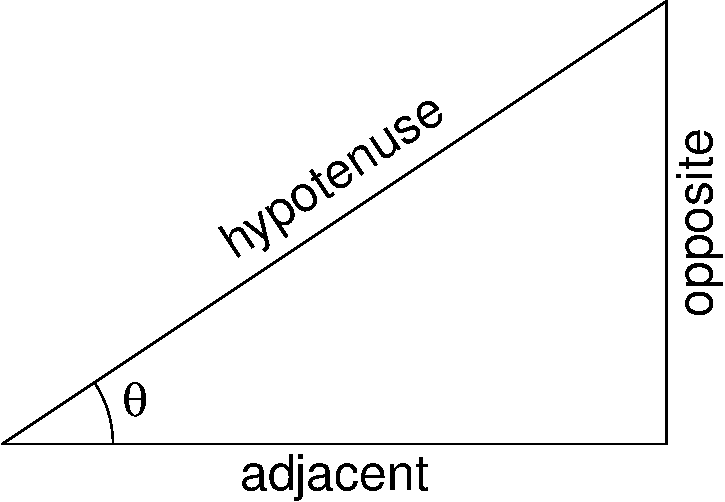
\includegraphics[width=0.5\linewidth]{PreCalculus-12-Minibook_files/figure-latex/trangle-1} \end{center}

    \end{col}

    \end{cols}
  \item
    The three trigonometric ratios of any angles, using the idea of the \href{https://www.miracleeducation.ca/PreCalculus-11-Minibook/trigonometry.html\#unitcircle}{unit circle}.
  \end{itemize}
\end{itemize}

\hypertarget{order-of-operations}{%
\subsection{Order of Operations}\label{order-of-operations}}

\begin{itemize}
\tightlist
\item
  Evaluating or simplifying an expression could involve multiple steps of operations. Generally, there are 4 levels of priorities:

  \begin{enumerate}
  \def\labelenumi{\arabic{enumi}.}
  \tightlist
  \item
    Parentheses
  \item
    Exponentiation
  \item
    Multiplication, Division
  \item
    Addition, Subtraction
  \end{enumerate}
\item
\end{itemize}

\hypertarget{use-of-parathesis}{%
\subsection{Use of Parathesis}\label{use-of-parathesis}}

\hypertarget{unary-and-binary-operations}{%
\subsection{Unary and Binary Operations}\label{unary-and-binary-operations}}

\hypertarget{inverse-operations}{%
\subsection{Inverse Operations}\label{inverse-operations}}

\hypertarget{algebra}{%
\section{Algebra}\label{algebra}}

\hypertarget{common-identities-and-simplification}{%
\subsection{Common Identities and Simplification}\label{common-identities-and-simplification}}

\hypertarget{solving-equations}{%
\subsection{Solving Equations}\label{solving-equations}}

\hypertarget{inequlities}{%
\subsection{Inequlities}\label{inequlities}}

\hypertarget{convensions-on-using-letters}{%
\subsection{Convensions on Using Letters}\label{convensions-on-using-letters}}

\hypertarget{functions}{%
\section{Functions}\label{functions}}

\hypertarget{introduction}{%
\subsection{Introduction}\label{introduction}}

\hypertarget{direct-and-inverse-proportionalities}{%
\subsection{Direct and Inverse Proportionalities}\label{direct-and-inverse-proportionalities}}

\hypertarget{linear-functions}{%
\subsection{Linear Functions}\label{linear-functions}}

\hypertarget{quadratic-functions}{%
\subsection{Quadratic Functions}\label{quadratic-functions}}

\hypertarget{analytic-geometries}{%
\section{Analytic Geometries}\label{analytic-geometries}}

\hypertarget{the-cartesian-plane}{%
\subsection{The Cartesian Plane}\label{the-cartesian-plane}}

\hypertarget{distance-between-points}{%
\subsection{Distance Between Points}\label{distance-between-points}}

\hypertarget{function-transformations}{%
\chapter{Function Transformations}\label{function-transformations}}

Looks like this chapter is not finished yet\ldots{}

\hypertarget{polynomials-and-polynomial-functions}{%
\chapter{Polynomials and Polynomial Functions}\label{polynomials-and-polynomial-functions}}

Looks like this chapter is not finished yet\ldots{}

\hypertarget{rational-radical-and-absolute-value-functions}{%
\chapter{Rational, Radical, and Absolute Value Functions}\label{rational-radical-and-absolute-value-functions}}

Looks like this chapter is not finished yet\ldots{}

\hypertarget{exponenetial-and-logarithmic-fucnitons}{%
\chapter{Exponenetial and Logarithmic Fucnitons}\label{exponenetial-and-logarithmic-fucnitons}}

Looks like this chapter is not finished yet\ldots{}

\hypertarget{geometric-sequences-and-series}{%
\chapter{Geometric Sequences and Series}\label{geometric-sequences-and-series}}

Looks like this chapter is not finished yet\ldots{}

\hypertarget{trigonometric-functions}{%
\chapter{Trigonometric Functions}\label{trigonometric-functions}}

Looks like this chapter is not finished yet\ldots{}

\hypertarget{trigonometric-identities}{%
\chapter{Trigonometric Identities}\label{trigonometric-identities}}

Looks like this chapter is not finished yet\ldots{}

\hypertarget{conics}{%
\chapter{Conics}\label{conics}}

Looks like this chapter is not finished yet\ldots{}

\hypertarget{other-topics}{%
\chapter{Other Topics}\label{other-topics}}

Looks like this chapter is not finished yet\ldots{}

\end{document}
